\subsection{DAC Control} \label{subsec:DAC_CONTROL} 
Section \refq{ch:SysArchitecture} shows that the the Sample Controller is responsible for controlling the DAC such that a stable sine wave is generated. The logic responsible for this will be described in this section. The specific section of the Sample Controller that handles the DAC logic is referred to as the DAC Control. A block diagram of the DAC Control can be seen on figure \refq{fig:7_2_3_DAC_CONTROL}.

\begin{figure}[H]
    \centering
    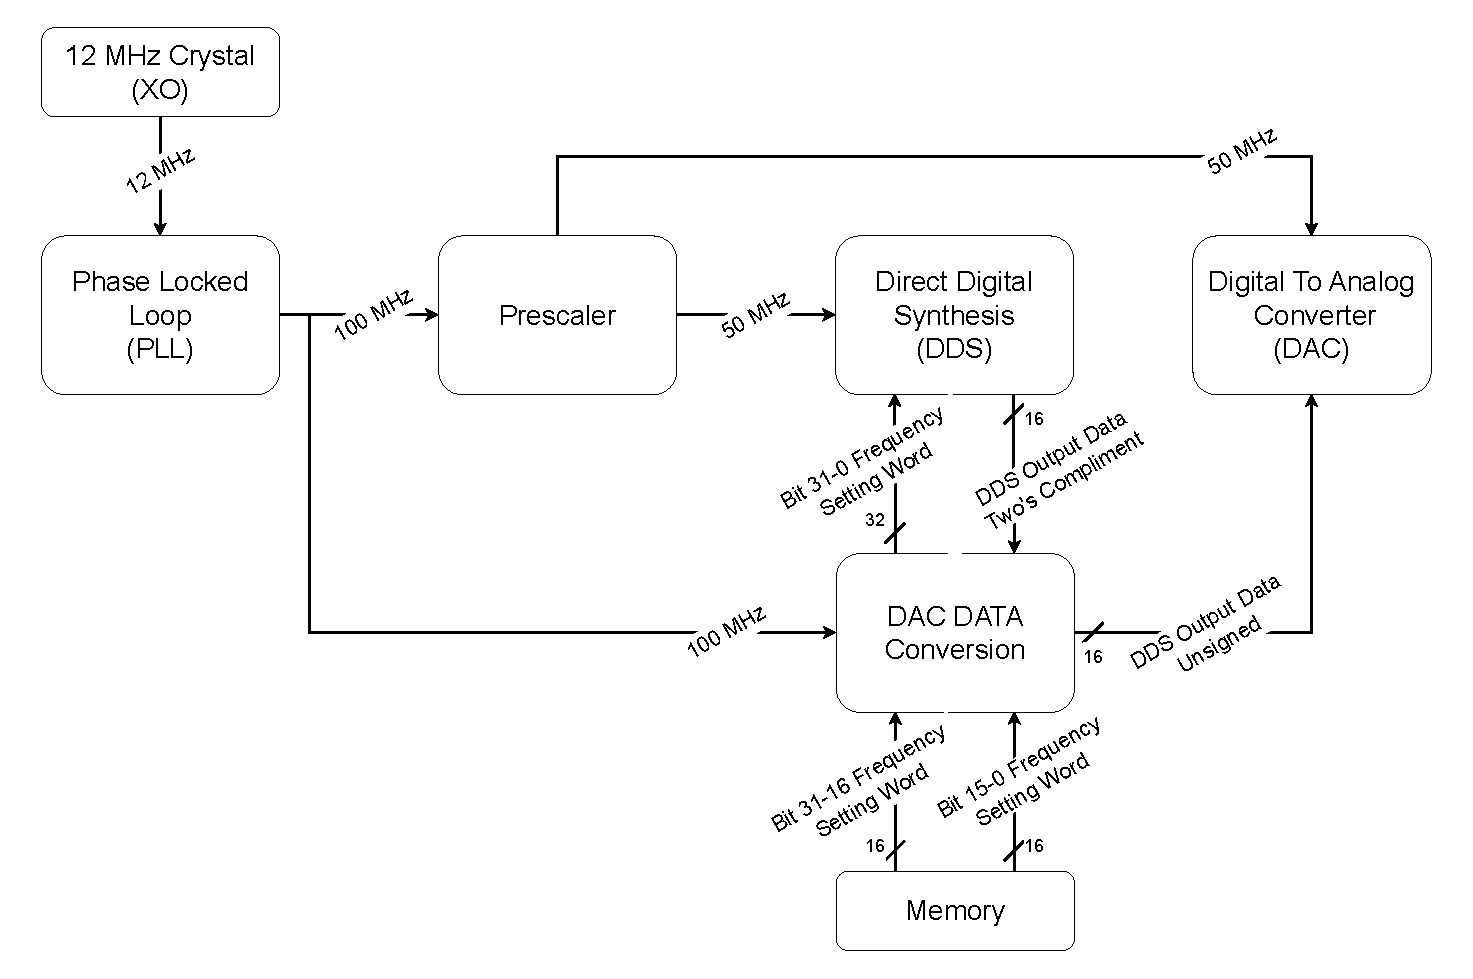
\includegraphics[clip, trim=0 0 0 0, width=1\textwidth]{Sections/7_SystemDesign/Figures/7_2_3_DAC_CONTROL.pdf}
    \caption{Block diagram of the DAC Control logic, the DAC is on the Analog Front End, it is shown here for completeness.}
    \label{fig:7_2_3_DAC_CONTROL}
\end{figure}

There are numerous of ways to generate sine waves, for this project a digital implementation has been favored due to the precise resolution that it offers. Requirement §1 from section \refq{ch:SystemRequirements} states that the frequency resolution must be at least \SIQ{1}{\hertz}. To achieve this, a Direct Digital Synthesis (DDS) principle has implemented. This essentially allows for a frequency resolution that is the DAC update rate divided by the length of the frequency setting word \cite{Fundamentals_DDS}. With a 32 bit wide frequency setting word, as specified by requirement §6.3.13 in section \refq{subsec:SampleControlSpec}, the resulting frequency resolution would be $f_{res} = \frac{DAC_{CLK}}{2^{32}}$.

The used DAC is an LTC1668, capable of an update rate of \SIQ{50}{\mega\hertz}. This essentially allows for a frequency resolution of \SIQ{11.6415}{\milli\hertz}, see equation \refq{eq:7_2_3_resolution}, assuming an update rate of \SIQ{50}{\mega\hertz}.

\begin{equation}
    \label{eq:7_2_3_resolution}
    f_{res} = \frac{\SIQ{50}{\mega\hertz}}{2^{32}} \Rightarrow \SIQ{11.6415}{\milli\hertz}. 
\end{equation}

Xilinx offers a complete "drag and drop" DDS block. The project team has settled on using this as it supports DAC resolutions of up to 18 bits and frequency setting words up to 48 bits, essentially making it ideal for the required DAC Control block. The principle of Direct Digital Synthesis will not be explained in this document, as it is not part of the scope of the project.

The DDS block is configured to take in a 32 bit wide frequency setting word, a \SIQ{50}{\mega\hertz} clock, and a frequency update signal. The output of the DDS block is configured for a 16 bit wide sine approximation as two's compliment.

All other blocks than the DDS shown in figure \refq{fig:7_2_3_DAC_CONTROL} are essentially there to "support" the DDS block. A \SIQ{50}{\mega\hertz} clock is generated via a Phase Locked Loop (PLL) and a prescaler. The PLL outputs a \SIQ{100}{\mega\hertz} signal that is divided by two and fed to the DDS block. The prescaler will also generate a \SIQ{50}{\mega\hertz} pulse train that is delayed from the DDS clock signal. This delayed pulse train is used to update the DAC and to detect if a new frequency setting word is present. The PLL is an integrated solution from Xilinx, much like the DDS block, and as such it will not be explained further.

The 16 bit wide output data of the DDS contains an approximated full-scale sine wave in two's compliment. The DAC however requires unsigned values as an input, and thus the DDS output data must be converted to a 16 bit wide unsigned bus. Furthermore the memory holds data in 16 bit registers, meaning that the 32 bit frequency setting word must be two registers that are concatenated. The DAC DATA Conversion block handles this concatenation and conversion from two's compliment to unsigned.

\subsection{DDS and DAC Prescaler}
The Prescaler for the DAC and DDS works much like a simple D flip flop. The VHDL code can be seen in listing \ref{lst:7_2_3_DAC_Prescaler}. 

\lstinputlisting[language=c ,style = c,firstnumber=1, linerange=34-59, caption={Code for DDS and DAC prescaler}, label={lst:7_2_3_DAC_Prescaler}]{Sections/7_SystemDesign/Code/DAC_PRESCALER.vhd}

When a rising edge of the master clock occurs on CLK\_IN, the output, called CLK\_TO\_DDS is inverted, essentially toggling it. This operation results in a divide by two behaviour, consequently meaning that the CLK\_TO\_DDS will have a frequency of half the CLK\_IN. The delayed pulse used to update the DAC is generated by anding the DDS clock and the inverted input clock. The different signals can be seen in figure \refq{fig:7_2_3_DAC_PRESCALER}.

\begin{figure}[H]
    \centering
    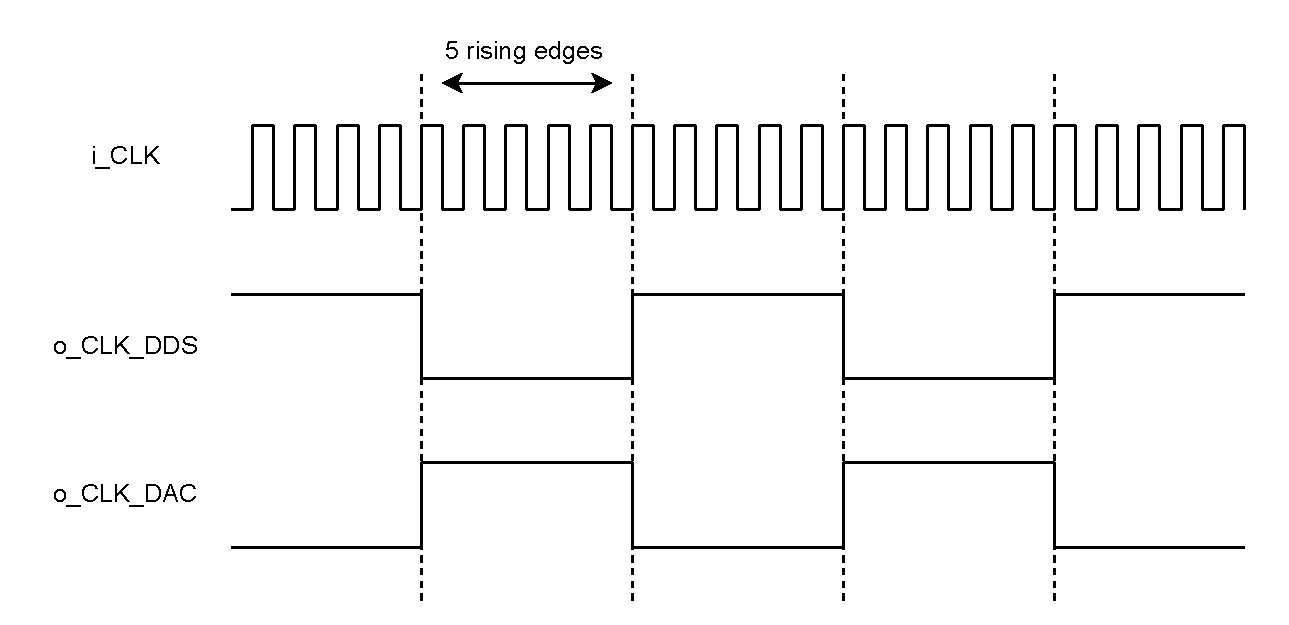
\includegraphics[clip, trim=0 0 0 0, width=1\textwidth]{Sections/7_SystemDesign/Figures/DAC_PRESCALER.pdf}
    \caption{Timing diagram of the input clock and output signals of the DDS and DAC Prescaler.}
    \label{fig:7_2_3_DAC_PRESCALER}
\end{figure}

The reasoning for generating a delayed pulse for the DAC is that the DDS will update its output value when a rising edge of the CLK\_TO\_DDS occurs, the output of the DDS will however need a few nano seconds to settle. To ensure that the DAC updates it output when correct data is present on its data-pins, it is good practice to let the data-pins have settled, thus by using a delayed pulse to clock the DAC, the data-pins are allowed more time to settle.

\subsection{DAC DATA Conversion}
The DAC DATA Conversion block ensures that the DAC is fed appropriate data and that the DDS block receives the proper 32 bit wide frequency setting word, as well as indicating to the DDS that new data is available for the frequency setting. The VHDL code for the DAC DATA Conversion can be seen in listing \refq{lst:7_2_3_DAC_DATA_Conversion}.

\lstinputlisting[language=c ,style = c,firstnumber=1, linerange=34-72, caption={Code for DAC DATA Conversion}, label={lst:7_2_3_DAC_DATA_Conversion}]{Sections/7_SystemDesign/Code/DAC_DATA_Conversion.vhd}

Lines 1 through 3 in listing \refq{lst:7_2_3_DAC_DATA_Conversion}, shows that it takes in SET\_F\_IN\_H and SET\_F\_IN\_L, and puts out F\_OUT. The two inputs are both 16 bit wide busses and the output F\_OUT is a 32 bit wide bus. Line 21 in the same list shows how the two inputs, SET\_F\_IN\_H and SET\_F\_IN\_L, are concatenated to form the 32 bit output bus F\_OUT.

The DAC DATA Conversion also takes in DDS\_DATA\_IN and outputs DAC\_DATA\_OUT, line 5 and 6 in list \refq{lst:7_2_3_DAC_DATA_Conversion}. Line 25 shows that DAC\_DATA\_OUT is rather simply DDS\_DATA\_IN xor'ed with the hex value "8000" or rather 32768 in decimal. This is the MSB value, and it results in the two's compliment data from the DDS being converted to unsigned values.

To see the effect of xor'ing two's compliment with the MSB, an example of the same operation with a 3 bit variable is shown in table \refq{tab:7_2_3_DAC_DATA_Conversion}. Here it can be seen that the result is that all values are offset by the value of the MSB, in the case of a 3 bit variable, it results in all values being offset by 4, or all values are added a value of 4. 

This is exactly what is desired, as the DAC output should be centered around an offset value, as the DAC cannot output negative values.

\begin{table}[H]
    \begin{tabular}{|l|l|l|l|}
    \hline
    \begin{tabular}[c]{@{}l@{}}A\\ Decimal\end{tabular} & \begin{tabular}[c]{@{}l@{}}A\\ 2's Comp\end{tabular} & B = A xor 100 & \begin{tabular}[c]{@{}l@{}}B\\ Decimal\end{tabular} \\ \hline
    3                                                   & 011                                                  & 111       & 7                                                           \\ \hline
    2                                                   & 010                                                  & 110       & 6                                                           \\ \hline
    1                                                   & 001                                                  & 101       & 5                                                           \\ \hline
    0                                                   & 000                                                  & 100       & 4                                                           \\ \hline
    -1                                                  & 111                                                  & 011       & 3                                                           \\ \hline
    -2                                                  & 110                                                  & 010       & 2                                                           \\ \hline
    -3                                                  & 101                                                  & 001       & 1                                                           \\ \hline
    -4                                                  & 100                                                  & 000       & 0                                                           \\ \hline
    \end{tabular}
    \caption{Example of two's compliment, A, xor'ed with the MSB of a 3 bit integer. The result is in the form of an unsigned integer
    0 having been offset by the value of the MSB.}
    \label{tab:7_2_3_DAC_DATA_Conversion}
    \end{table}

    The process in line 27 trough 37 in listing \refq{lst:7_2_3_DAC_DATA_Conversion} shows how the logic detects if the frequency setting words has been updated. When a rising edge of the CLK\_IN, here the same clock that drives the DAC, takes place, the input data sig\_f\_in and latched output data sig\_f\_out are compared, if they are not the same, the logic will set sig\_update\_f to high, and update the latched output data to match the input data. On the next rising edge of CLK\_IN, the data will be the same, and here sig\_update\_f is then set to low again. This creates a pulse the length of the period of CLK\_IN, only when new data is present on sig\_f\_in. 
    
    The DDS block will update its output frequency when a rising edge appears on its update frequency input, and thus the DDS will only update its output frequency when new data is present on sig\_f\_in, and sig\_f\_in is generated from concatenating the two memory registers containing the DAC frequency, resulting in the DDS only updating its frequency when the MCU programs in a new frequency to the memory.